\chapter{Fundamentação teórica}
\label{cap:fundamentacao-teorica}

Entender o comportamento de sequencias de eventos ao longo do tempo e como eventos influenciam uns aos outros requer o uso de ferramentas matemáticas complexas. Este capitulo irá apresentar a fundamentação teórica necessária para suportar o modelo proposto. Vamos começar com a distribuição de Poisson e a modelagem de processos pontuais, necessárias para entender como eventos acontecem em tempo contínuo de forma irregular. Em seguida, veremos Processo de Hawkes, que mostra como eventos podem afetar a probabilidade de eventos futuros. Depois, apresentamos os processos de Hawkes neurais, que substituem o kernel paramétrico por redes neurais, culminando no \textit{Neural Hawkes Process}, e revisamos a arquitetura Transformer e seu mecanismo de atenção. As abordagens de processos de Hawkes baseadas em Transformers (THP e RoTHP) e as técnicas de extrapolação de comprimento, que são a base direta do modelo proposto, são tratadas no Capítulo~\ref{cap:trabalhos-relacionados}.

\section{Distribuição de Poisson}\label{sec:distribuicao-de-poisson}

    Antes de tratarmos do Processo de Poisson, convém relembrar a distribuição de Poisson, da qual ele herda o nome. A distribuição de Poisson é uma distribuição de probabilidade discreta que modela o número de eventos que ocorrem em um intervalo fixo (de tempo, espaço, etc.), supondo que esses eventos sejam independentes e aconteçam a uma taxa média constante $\lambda$. A probabilidade de observar exatamente $k$ eventos é dada por:
    \begin{equation}
        \Pr(X = k) = \frac{\lambda^{k} e^{-\lambda}}{k!}, \quad k = 0, 1, 2, \ldots,
        \label{eq:distribuicao-poisson}
    \end{equation}
    onde $\lambda > 0$ é o número médio de eventos esperado no intervalo. Uma propriedade marcante dessa distribuição é que sua média e sua variância são ambas iguais a $\lambda$: quanto maior a taxa, mais eventos esperamos e maior a variabilidade em torno desse valor.

    Na próxima seção veremos que o Processo de Poisson é justamente o mecanismo que gera eventos ao longo do tempo de modo que a contagem em qualquer intervalo siga essa distribuição. Lá, a Equação~\ref{eq:poisson} reaparece com $\Lambda = \lambda T$ no lugar de $\lambda$, indicando que o número esperado de eventos cresce proporcionalmente ao tamanho $T$ do intervalo observado.


\section{Processos de Poisson}\label{sec:processos-de-poisson}

    O Processo de Poisson é um objeto matemático que consiste de pontos aleatórios em um espaço matemático com a importante característica de não dependência entre os pontos. Esse modelo é amplamente utilizado em áreas como teoria das filas, astronomia, biologia e análise de sobrevivência. O nome deriva do fato de que os pontos, ou eventos, ocorrem seguindo uma distribuição de Poisson.
    
    Processo de Poisson é a forma mais comum de Processos Pontuais. \citeonline{daley_introduction_2003} definem um Processo de Poisson estacionário pela equação a seguir, onde usamos $N(a_i, b_i]$ para representar o número de eventos do processo. 
    \begin{equation}
        \Pr\{N((a_i, b_i]) = n_i,\; i = 1, \ldots, k\}
        = 
        \prod_{i=1}^{k}
        \frac{[\lambda (b_i - a_i)]^{n_i}}{n_i!}\,
        e^{-\lambda (b_i - a_i)}.
        \label{eq:start-poisson}
    \end{equation}

    Esta definição engloba três aspectos importantes: $(\mathrm{i})$ o número de pontos em cada intervalo finito $(a_i,b_i]$ possui uma distribuição de Poisson; $(\mathrm{ii})$ o número de pontos em intervalos disjuntos são variáveis aleatórias independentes; e $(\mathrm{iii})$ as distribuições são estacionárias, ou seja, dependem apenas dos comprimentos $b_i-a_i$ dos intervalos. A constante $\lambda$ é a taxa média ou a densidade média dos eventos do processo. Nas subseções a seguir veremos que $\lambda$ é também a intensidade com a qual os eventos ocorrem.

    Considerando o caso especial de apenas um intervalo $k=1$, temos  $(a_i, b_i] = (0,T]$. Então, o tamanho do intervalo é $b_i-a_i=T$. Substituindo na Equação \ref{eq:start-poisson}, temos: 

    \begin{equation}
        \Pr\{N((0,T]) = n_1\}
        = \frac{[\lambda T]^{n_1}}{n_1!}\,
        e^{-\lambda T}.
        \label{eq:poisson-lambda}
    \end{equation}
        
    Na Equação \ref{eq:poisson-lambda}, substituindo $(0,T]$ por $N$ e $\lambda T$ por $\Lambda$, temos a forma clássica da distribuição de Poisson associada ao Processo de Poisson:
    \begin{equation}
        \Pr(N = n)
        =
        \frac{\Lambda^{n}}{n!}\, e^{-\Lambda}.
        \label{eq:poisson}
    \end{equation}

    A Equação \ref{eq:poisson} explicita a relação entre a distribuição de Poisson e o Processo de Poisson: o numero de eventos observados em qualquer intervalo de tamanho T é Poisson com a média $\Lambda = \lambda T$. Em outras palavras, o Processo de Poisson é uma forma de gerar tempos de eventos cuja contagem satisfaz a distribuição de Poisson e que sejam independentes e estacionários. Processos de Poisson são a forma mais fundamental de Processos Pontuais Temporais, que iremos falar na próxima seção. 

    A Figura \ref{fig:poisson} ilustra um Processo de Poisson homogêneo no intervalo $[0,T]$. O eixo horizontal representa o tempo e cada traço vertical representa a ocorrência de um evento gerado pelo processo. Embora os eventos pareçam irregulares, eles foram gerados de modo que o tempo de espera entre um evento e outro seja exponencial $1/\lambda$ e independente, onde $\lambda$ é constante e portanto o número de eventos esperado em um determinado intervalo $T$ é definido por $\lambda T$. Isso ilustra a intuição por trás do processo de Poisson que é a ocorrência aleatória de eventos, independentes e seguidos por uma taxa constante $\lambda$.
    
    \begin{figure}[h!]
		\centering
		\captionsetup{width=14cm}%Da mesma largura que a figura
		\Caption{\label{fig:poisson}Processo de Poisson.}        
		\UFCfig{}{
			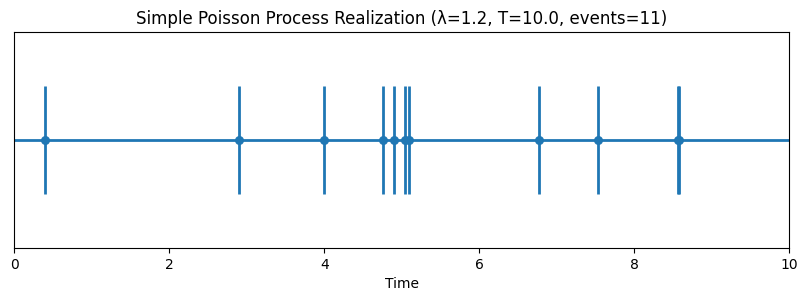
\includegraphics[width=14cm]{figuras/figura-poisson.png}
		}{
			}	
	\end{figure}

\section{Processos Pontuais Temporais}\label{sec:processos-pontuais-temporais}

    Processos Pontuais Temporais (TPP) são modelos probabilísticos desenhados para descrever sequências de eventos discretos que acontecem em tempo contínuo \cite{zuo_transformer_2021}. Diferentemente de modelos discretos, que assumem que os eventos acontecem em intervalos de tempo conhecidos, TPPs permitem lidar com eventos que acontecem em tempos irregulares, arbitrários. Isso os tornam particularmente uteis em domínios onde o momento da ocorrência do evento é tão importante quanto o evento em si. 

    Muitas cenários geram tais sequências de eventos, desde de picos de neurônios em neurociência, compra e venda de ações no mercado financeiro, tuítes em redes sociais, etc \cite{zhou_advances_2025}. Essas sequências de eventos, composta por eventos assíncronos, geralmente influenciam uns aos outros, tornando o estudo desses fenômenos não apenas complexo como também necessário. 

    Os TPPs são formalmente definidos por uma função de intensidade condicional $\lambda(t \mid \mathcal{H}_t)$, onde $\mathcal{H}_t$ é o histórico de eventos até o tempo $t$. A intensidade é a taxa instantânea pela qual espera-se que um evento ocorra em um tempo $t$, dado os eventos passados.

    Uma variação dos TPPs é a existência de \textit{marcas}, ou seja, tipos de eventos, onde a sequência passa a ser descrita como $X = \{(t_1, m_1), \ldots, (t_N, m_N)\}$, onde $N$ representa o número de eventos e cada $m_i$ é a marca (tipo) associado ao evento $i$. 

    A distribuição de um TPP com marcas $K$ pode ser caracterizado por $K$ funções de intensidade condicionais $\lambda_k(t \mid \mathcal{H}_t)$ (uma para cada marca $k$) e é definida como 
    \begin{equation}
        \lambda_k(t \mid \mathcal{H}_t)
        = \lim_{\Delta t \to 0}
        \frac{
        \Pr(\text{evento do tipo } k \text{ em } [t, t + \Delta t) \mid \mathcal{H}_t)
        }{
        \Delta t
        }.
    \end{equation}
    Perceba que a definição acima também pode ser aplicada para TPPs sem marcas, apenas definindo $K = 1$ \cite{shchur_neural_2021}.

    \subsection{Função custo}\label{sec:funcao-custo}

    Para processos pontuais, dada a observação de todos os eventos no intervalo $[0,T]$, utilizamos o logaritmo da verissimilhança conforme equação abaixo: 
    \begin{equation}
        \mathcal{L} = \sum_{i:t_i \leq T} \log \lambda_{k_i}(t_i) - \underbrace{\int_{t=0}^{T} \lambda(t)dt}_{\text{Chamemos de $\Lambda$}}. \label{eq:log_likelihood_final}
    \end{equation}

    Vamos derivar esta função de acordo com \citeonline{mei_neural_2017}. Primeiro, define-se $N(t) = |\{h : t_h \leq t\}|$ como a contagem de eventos (de qualquer tipo) anteriores ao tempo $t$. Dado o histórico passado $\mathcal{H}_i$, o número de eventos em $(t_{i-1}, t]$ é $\Delta N (t_{i-1}, t) \overset{\text{def}}{=} N(t) - N(t_{i-1})$.
    
    Seja $T_i > t_{i-1}$ a variável aleatória do tempo do próximo evento e $K_{i+1}$ a variável aleatória do tipo do próximo evento. A função de distribuição cumulativa e a função densidade de probabilidade de $T_i$ (condicionada a $\mathcal{H}_i$) são dadas por:
    \begin{align}
        F(t) &= P(T_i \leq t) = 1 - P(T_i > t) \\
        &= 1 - P(\Delta N (t_{i-1}, t) = 0) \\
        &= 1 - \exp \left( - \int_{t_{i-1}}^{t} \lambda(s)ds \right) \\
        &= 1 - \exp (\Lambda(t_{i-1}) - \Lambda(t)) \label{eq:cdf_4} \\
        f(t) &= exp(\Lambda(t_{t-1})-\Lambda(t))\lambda(t),
    \end{align}
    onde $\Lambda(t) = \int_{0}^{t} \lambda(s)ds$ e $\lambda(t) = \sum_{k=1}^K \lambda_k(t)$.
        
    Além disso, dado o histórico passado $\mathcal{H}_i$ e o tempo do próximo evento $t_i$, a distribuição do tipo de evento $k_i$ (probabilidade de ser do tipo $k_i$) é dada por:
    \begin{equation}
        P (K_i = k_i \mid t_i = \frac{\lambda_{k_i}(t_i)}{\lambda(t_i)} \label{eq:cond_type_prob}
    \end{equation}
    
    Portanto, podemos derivar a função de verossimilhança $L$ assim:
    \begin{align}
        L &= \prod_{i:t_i \leq T} L_i \\ 
        &= \prod_{i:t_i \leq T} \{ f(t_i) P(K_i = k_i \mid t_i) \} \label{eq:likelihood_prod_1} \\
        &= \prod_{i:t_i \leq T} \left\{ \exp (\Lambda(t_{i-1}) - \Lambda(t_i)) \lambda_{k_i}(t_i) \right\} \label{eq:likelihood_prod_3}
    \end{align}
    
    Finalmente, ao aplicar o logaritmo na verossimilhança transformamos o produto em soma:    
    \begin{align}
        \mathcal{L} &\overset{\text{def}}{=} \log L \\
        &= \sum_{i:t_i \leq T} \log\lambda_{k_i}(t_i)-\sum_{i:t_i \leq T}(\Lambda (t_i)-\Lambda(t_{i-1})) \\
        &= \sum_{i:t_i \leq T} \log \lambda_{k_i}(t_i) - \Lambda(T) \label{eq:log_likelihood_final_2} \\
        &= \sum_{i:t_i \leq T} \log \lambda_{k_i}(t_i) - \int_{t=0}^{T} \lambda(t)dt \label{eq:log_likelihood_final_3}
    \end{align}

\section{Processos de Hawkes}\label{sec:processos-de-hawkes}

    Processos de Poisson são uma forma básica de trabalhar com sequências de eventos discretos, porém, parte-se do principio de que tais eventos são independentes uns dos outros. Mesmo em um processo de Poisson multivariado e não homogêneo, onde a variação da probabilidade da ocorrência de um evento em $t$ varia em função de $t$, ainda assim os eventos são independentes entre si. Ele assume que um evento do tipo $k$ acontece no intervalo infinitesimal $[t,t+\mathrm{d}t]$, com probabilidade $\lambda_k(t)\mathrm{d}t$. A intensidade total de todos os eventos é data por $\lambda(t)=\sum_{k=1}^{K}\lambda_k(t)$.
    
    Já o Processo de Hawkes parte do princípio de que eventos passados influenciam a probabilidade de eventos futuros. Em um Processo de Hawkes tradicional, supomos que essa probabilidade é sempre aumentada, somada à probabilidade de eventos passados e decai exponencialmente \cite{mei_neural_2017}.

    O Processo de Hawkes é considerado duplamente estocástico \cite{zuo_transformer_2021}, pois  $\lambda(t)$ é uma variável aleatória, como em um processo de Cox, mas também é um processo de Poisson. A intensidade de um Processo de Hawkes tradicional univariado é dada por:
    \begin{equation}        
        \lambda(t \mid \mathcal{H}_t)= \mu+        \sum_{t_i < t}\alpha\, e^{-\beta (t - t_i)}, 
        \label{eq:hawkes}
    \end{equation}

    onde $\alpha$ representa o aumento na intensidade de probabilidade instantâneo causado por pelo evento $e$ e $\beta$ representa a velocidade com que essa intensidade decai ao londo do tempo.

    A Figura \ref{fig:hawkes} ilustra a intensidade de probabilidade $\lambda$ de um evento onde do $t = 0$ até $t = 2$ essa intensidade está estacionada em uma basaline $\mu$. No momento $t = 2$, acontece o evento $e$, elevando a intensidade de probabilidade instantaneamente. Em seguida, $\lambda$ decai exponencialmente, voltando para o estado  estacionário $\mu$, que representa a não influência de nenhum evento no momento $t$.
    
	\begin{figure}[h!]
		\centering
		\captionsetup{width=14cm}%Da mesma largura que a figura
		\Caption{\label{fig:hawkes}Função de intensidade de probabilidade}{Função de intensidade de probabilidade representando auto excitação instantânea e decaimento exponencial.}	
		\UFCfig{}{
			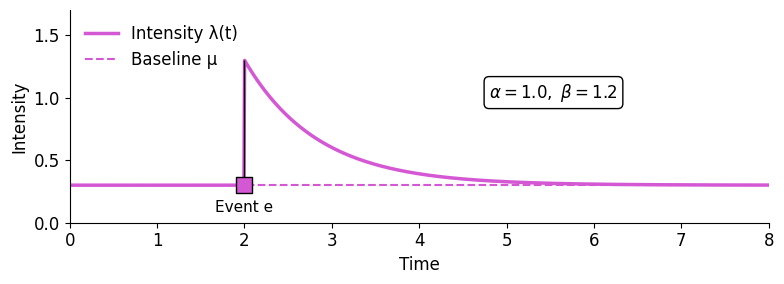
\includegraphics[width=14cm]{figuras/figura-hawkes.png}
		}{
			}	
	\end{figure}

    Ao longo deste trabalho iremos considerar o Processo de Hawkes multivariado, que é capaz de capturar a influencia de eventos de diferentes tipos $k$ entre si, como uma postagem em uma rede social influenciar positivamente a ocorrência de um outro tipo de interação, ou evento neurológico ser gatilho para um determinado acidente cerebral.

    \subsection{Relação com o Processo de Cox}\label{subsec:processo-de-cox}

    Vale situar o Processo de Hawkes dentro de uma progressão de modelos de intensidade cada vez mais flexíveis. No Processo de Poisson homogêneo, a intensidade $\lambda$ é constante. No Processo de Poisson não homogêneo, ela passa a variar no tempo de forma determinística, $\lambda(t)$. Um passo além é o \textbf{Processo de Cox}, também chamado de Processo de Poisson duplamente estocástico, no qual a própria intensidade $\lambda(t)$ é um processo aleatório, governado por fatores externos ao histórico de eventos.

    O Processo de Hawkes pode ser visto como um caso particular dessa ideia de intensidade estocástica: a aleatoriedade de $\lambda(t)$ não vem de uma fonte externa, mas dos próprios eventos passados, cada um elevando temporariamente a probabilidade de novos eventos (Equação~\ref{eq:hawkes}). É nesse sentido que o Processo de Hawkes é descrito como duplamente estocástico, como mencionado anteriormente. Neste trabalho, é justamente essa dependência do histórico (e o decaimento exponencial da influência de eventos passados) que motiva o viés de recência do modelo proposto.

\section{Processos Pontuais Temporais Neurais}\label{sec:processos-pontuais-temporais-neurais}

    Vimos que Processos de Hawkes descrevem muitos cenários, porém, a sua forma clássica não contempla as complexidades do dia a dia, intrínsecas à muitos eventos. Eventos podem possuir uma influência inibitória, ao invés de excitatória, sobre outros eventos, como, por exemplo, uma manutenção preventiva diminui a probabilidade de ocorrência de uma falha em um equipamento. Outra premissa dos processos de Hawkes tradicionais é considerar que eventos do mesmo tipo possuem influência constante sobre outros eventos, porém, sabemos que, por exemplo, ao assistir um fenômeno pela vigésima vez nosso cérebro é menos excitado do que quando presenciamos o evento pela primeira vez. Por fim, podemos também lembrar de fenômenos onde a influência sobre outros eventos não decai de forma exponencial \cite{mei_neural_2017}.

    \citeonline{mei_neural_2017} mencionam como é dificil aplicar o processo de Hawkes tradicional em cenários com dados faltantes. Até mesmo em domínios onde Hawkes seria apropriado, a própria natureza dos dados pode apresentar desafios, tais como sequências parcialmente observadas ou dados omitidos de forma sistemática. Existem também dados omitidos de forma estocástica, que podem ser bastante complexos para a versão tradicional de Hawkes.

    Para resolver tais limitações do processo de Hawkes, abordagens utilizando redes neurais foram propostas, sendo o de \citeonline{mei_neural_2017} um dos trabalhos mais difundidos e aceitos pela comunidade, onde propuseram o \gls{NHP}.

    O primeiro passo foi relaxar a regra de manter $\alpha$ e $\mu$ estritamente positivos, e isso fez com que os valores orbitassem no $\mathbb{R}$, abordando inibição $(\alpha < 0)$ e inércia $(\mu < 0)$. Porém, agora o resultado pode ser negativo, o que não faria sentido para uma intensidade de probabilidade, então é necessário fazer uma transformação $f = \mathbb{R} \to \mathbb{R_+}$, fazendo $\lambda_k(t) = f_k(\tilde \lambda_k(t))$, onde $k$ é o tipo do evento. A função ReLU $f(x) = \mathrm{max}(x, 0)$ seria uma escolha natural para fazer essa conversão, porém, ela assume valor 0 para números negativos e a nossa intensidade precisa assumir valores sempre positivos quando houver possibilidade de um evento ocorrer. 
    
    A função escolhida, então, pelos autores foi a softplus $f(x) = s\mathrm{log}(1 + exp(x/s))$, onde $s$ é um parâmetro de escala aprendido introduzido pelo modelo para trazer estabilidade numérica, pois quando a unidade de $x$ varia, por exemplo, de segundos para milissegundos, a intensidade base $f(\mu_k)$ se torna mil vezes menor, forçando $\mu_k$ a assumir valore negativos e dessa forma criando um forte efeito de inércia. 

    O segundo passo foi remover a restrição de que eventos passados possuem independência e influência aditiva em $\lambda(t)$. Ao invés de prever $\lambda(t)$ utilizando o somatório do modelo paramétrico tradicional de Hawkes (Equação \ref{eq:hawkes}), \citeonline{mei_neural_2017} utilizaram uma rede neural recorrente, que permitiu capturarem padrões complexos, antes dificilmente percebidos em versões paramétricas do modelo.
    
    Como nos modelos tradicionais, cada tipo de evento $k$ possui uma densidade dependente do tempo $\lambda_k(t)$, que salta a cada novo evento e decai exponencialmente até um valor estacionário, análogo ao $\mu$ da Equação \ref{eq:hawkes}. Entretanto, no modelo proposto por \citeonline{mei_neural_2017} essa dinâmica é controlada por uma vetor de estados oculto $\mathbf{h}(t) \in (-1,1)^D$, que depende do vetor $\mathbf{c}(t) \in \mathbb{R}^D$, que é o vetor de memória de uma rede neural recorrente com uma camada e $D$ neurônios. 
    
    \citeonline{mei_neural_2017} propuseram uma variação da \gls{LSTM} para tempo continuo, a Continuous-Time LSTM (CT-LSTM), onde após cada evento cada célula de memória $c$ decai exponencialmente a uma determinada taxa $\mathbf{\delta}$ até um estado estável (estacionário) $\mathbf{\bar{c}}$. A cada momento em $t>0$, é possível obter a intensidade de cada tipo de evento com $\lambda_k(t)=f_k(\mathbf{w}_k^T\mathbf{h}(t))$, onde $\mathbf{h}$ pode ser calculado com $\mathbf{h}(t)=\mathbf{o}_i \odot (2\mathbf{\sigma}(2\mathbf{c}(t))-1$ para $t \in (t_{i-1},t_i]$, onde $\mathbf{o}$ é o vetor de saída (output) da LSTM e $\mathbf{w}$ um vetor de pesos. 
    \begin{align}
        \mathbf{i}_{i+1} &\leftarrow \sigma(\mathbf{W}_i \mathbf{k}_i+\mathbf{U}_i \mathbf{h}(t_i)+\mathbf{d}_i) \label{eq:neural-i} \\
        \mathbf{f}_{i+1} &\leftarrow \sigma(\mathbf{W}_f \mathbf{k}_i+\mathbf{U}_f \mathbf{h}(t_i)+\mathbf{d}_f) \label{eq:neural-f} \\
        \mathbf{z}_{i+1} &\leftarrow 2\sigma(\mathbf{W}_z \mathbf{k}_i+\mathbf{U}_z \mathbf{h}(t_i)+\mathbf{d}_z) - 1 \label{eq:neural-z} \\
        \mathbf{o}_{i+1} &\leftarrow \sigma(\mathbf{W}_o \mathbf{k}_i+\mathbf{U}_o \mathbf{h}(t_i)+\mathbf{d}_o) \label{eq:neural-o}
    \end{align}
    \begin{align}
        \mathbf{c}_{i+1} &\leftarrow \mathbf{f}_{i+1} \odot \mathbf{c}(t_i)+\mathbf{i}_{i+1} \odot \mathbf{z}_{i+1} \label{eq:neural-c} \\
        \mathbf{\bar{c}}_{i+1} &\leftarrow \mathbf{\bar{f}}_{i+1} \odot \mathbf{\bar{c}}_i+\mathbf{\bar{i}}_{i+1} \odot \mathbf{z}_{i+1} \label{eq:neural-cbar} \\
        \mathbf{\delta}_{i+1} &\leftarrow f(\mathbf{W}_d \mathbf{k}_i+\mathbf{U}_d \mathbf{h}(t_i)+\mathbf{d}_d) \label{eq:neural-delta}
    \end{align}

    As Equações \ref{eq:neural-i}, \ref{eq:neural-f} e \ref{eq:neural-o} referem-se respectivamente aos \textit{Gates} de \textit{input}, \textit{forget} e \textit{output}, comuns a uma rede LSTM convencional. A Equação \ref{eq:neural-z} refere-se ao valor candidato (\textit{Candidate Memory}). As Equações \ref{eq:neural-c} e \ref{eq:neural-cbar} representam a Célula de Memória (\textit{Memory Cell}) e o estado estável da Célula de Memória. Finalmente, a Equação \ref{eq:neural-delta} calcula o vetor $\mathbf{\delta}$, a taxa de decaimento, análogo ao $\beta$ da Equação \ref{eq:hawkes}.

    As equações acima se assemelham bastante a uma LSTM convencional (discreta), mas com duas diferenças fundamentais. As atualizações não dependem do valor anterior $t_{t-1}$ e sim do valor de $\mathbf{h}(t_i)$, após ele ter sofrido decaimento no período $t_i-t_{i-1}$. Além disso, as Equações \ref{eq:neural-cbar} e \ref{eq:neural-delta} são novas, adicionadas por \citeonline{mei_neural_2017}, e elas definem como, ao longo do tempo, à medida em que $t>t_i$ aumenta os elementos de $\mathbf{c}(t)$ irão continuamente decair de $\mathbf{c}_{i+1}$ até $\mathbf{\bar{c}}_{i+1}$. $\mathbf{c}(t)$ é calculado de acordo com a equação
    \begin{equation}
        \mathbf{c}(t) \overset{\text{def}}{=} \mathbf{\bar{c}}_{i+1} + (\mathbf{c}_{i+1}-\mathbf{\bar{c}}_{i+1}) \exp(-\mathbf{\delta}_{i+1}(t-t_i)) \quad \text{para } t \in (t_i,t_{i+1}].
        \label{eq:neural-ct}
    \end{equation}

    Importante lembrar que $\mathbf{c}(t)$ é utilizado na função $\mathbf{h}(t)$, que é análoga ao vetor do estado oculto $\mathbf{h}_i$ da LSTM, que, por sua vez, é utilizada no cálculo do $\lambda_k(t)$, para um determinado tipo de evento $k$. 
    
    A abordagem de \citeonline{mei_neural_2017} foi simples, mas bastante engenhosa, obtendo excelentes resultados tanto em datasets sintéticos como reais, sendo muitas vezes ainda o melhor benchmark, apesar de ser um algoritmo de 2017.

\section{Transformers e o mecanismo de atenção}\label{sec:transformers-atencao}

    Abordagens baseadas em redes neurais recorrentes (RNN), como a Continuous Time LSTM (CT-LSTM) proposta por \citeonline{mei_neural_2017} trouxe grandes avanços na modelagem de padrões complexos, porém, continuaram com o ponto fraco das RNNs que é o fato de seu processamento ser sequencial. RNNs processam um evento após o outro, ou seja, o calculo do evento próximo evento ($t_{i+1}$) depende do evento atual ($t_i$), fazendo com que o treino da rede seja lento. Em alguns cenários, de sequências muito longas, se torna inviável utilizar RNN. Trabalhos mais recente adaptaram a arquitetura Transformer proposta por \citeonline{vaswani_attention_2017}, adaptando o mecanismo de Atenção para TPP, especialemnte voltadas para o Processo de Hawkes, que é o foco deste trabalho. As subseções seguintes vão nos ajudar a relembrar como é a arquitetura proposta em 2017.

\subsection{Encoders e Decoders}\label{subsec:encoders-decoders}

    O Encoder é o componente responsável por processar a sequência de entrada e transformá-la em uma representação mais rica de informação. Ele é composto por $N$ camadas idênticas empilhadas (no modelo original de \citeonline{vaswani_attention_2017}, $N = 6$ e a dimensão dos vetores é $d_{model} = 512$, mas esses valores são hiperparâmetros que variam conforme a aplicação). Cada camada possui duas subcamadas: a primeira é a Multi-Head Self Attention, que calcula a relevância de cada input com relação aos demais inputs da sequência. A segunda é uma rede feed-forward completamente conectada, que aplica não linearidade para cada posição.

    De forma semelhante, o Decoder também é constituído por $N$ camadas empilhadas. Porém, para gerar o output, o Decoder utiliza uma terceira subcamada, que faz um Multi-Head Attention no output do Encoder, conectando o contexto processado pelo Encoder com a sequência gerada pelo Decoder. Além disso, o Decoder utiliza máscara para prevenir que o modelo compute posições futuras na sequência, fazendo com que cada predição considere apenas eventos conhecidos \cite{vaswani_attention_2017}.

\subsection{Mecanismo de Atenção}\label{subsec:mecanismo-de-atencao}

    A inovação principal introduzida pelo modelo é o mecanismo de atenção, também chamada de Scaled Dot-Product Attention, sem a necessidade de redes neurais recorrentes, que faz com que todas as entradas (eventos) sejam processados simultaneamente. Dessa forma o modelo consegue calcular a influência (atenção) de cada evento em relação aos demais eventos.

    Diferentemente das RNNs, que mantém apenas um vetor com o estado oculto $\mathbf{h}$, redes baseadas em Transformers calculam a influência de cada evento e calcula $\mathbf{h}$ através de uma soma ponderada, que, por sua vez, foi calculada com base na influência de cada evento, dentro do contexto da lista de eventos. 

    A entrada consiste de vetores de queries $Q$ e chaves $K$ de dimensão $d_k$ e valores $V$ de dimensão $d_v$. É calculado então o produto da query com todas as chaves, dividido cada um por $\sqrt{d_k}$ e então uma função softmax é aplicada para obter os pesos dos valores (dos vetores chave-valor). A matrix de outputs é calculada como
    \begin{equation}
        \text{Attention}(Q,K,V) = \text{softmax}(\frac{QK^T}{\sqrt{d_k}})V
        \label{eq:attention}.
    \end{equation}

\subsection{Multi-Head Attention}\label{subsec:multi-head-attention}

    Ao invés de performar apenas uma função de Atenção com Queries, Keys e Values de dimensão $d_{model}$, \citeonline{vaswani_attention_2017} decidiram projetar linearmente os vetores Q, K e V um número $h$ de vezes com projeções lineares diferentes e aprendidas para $d_k$, $d_k$ e $d_v$ dimensões, respectivamente. Para cada uma das versões projetadas de Q, K e V é executada a função de Atenção em paralelo, gerando outputs de $d_v$ dimensões. Os outputs são então concatenados e projetados novamente, gerando os valores finais, como mostra a equação abaixo:
    \begin{equation}
    \begin{split}
        \text{MultiHead}(Q,K,V) &= \text{Concat}(\text{head}_1, \dots, \text{head}_h)W^O \\
        &\quad \text{onde } \text{head}_i = \text{Attention}(QW_i^Q, KW_i^K, VW_i^V)
    \end{split}
    \label{eq:multi-head-attention}
    \end{equation}

    A Figura \ref{fig:attention} ilustra a diferença entre o mecanismo simples de atenção e o mecanismo de multi-head attention \cite{vaswani_attention_2017}.

    \begin{figure}[h!]
		\centering
		\captionsetup{width=14cm}%Da mesma largura que a figura
		\Caption{\label{fig:attention}Attention x Multi-Head Attention.}        
		\UFCfig{}{
			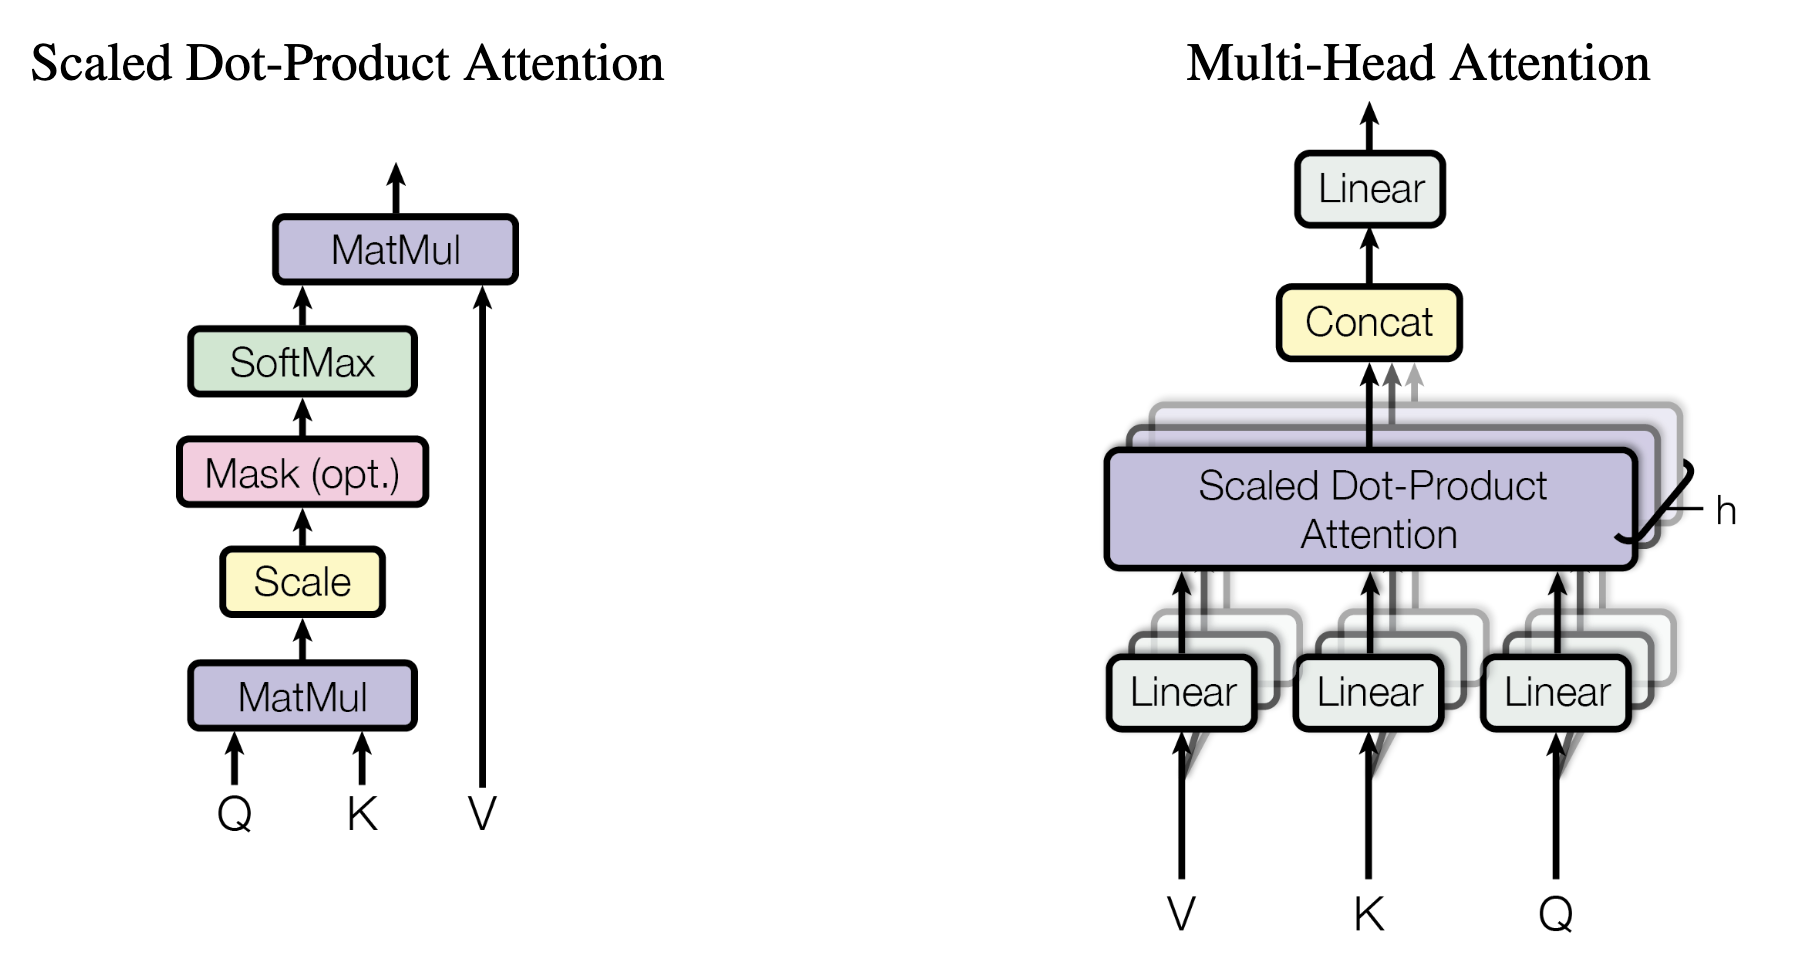
\includegraphics[width=14cm]{figuras/figura-attention.png}
		}{
			}	
	\end{figure}